\chapter*{Retos de Matemáticas Básicas}

\section*{Aritmética}

i). ¿Cuánto vale la siguiente multiplicación de fracciones?: $$\left(\frac{60}{21}\right)\times\left(\frac{1}{33}\right)\times\left(\frac{6}{5}\right)\times \left(\frac{35}{8}\right)$$\\

%Sug: 1. ¿Cómo se multiplican las fracciones?. 2. Factoriza y cancela (no se tiene que hacer ninguna multiplicación). Recuerda que el orden de los factores no altera el producto (tanto el de arriba como el de abajo). \\

ii). ¿Cuánto vale $$\left(\frac{1}{2}\right)\times\left(\frac{2}{3}\right)\times\left(\frac{3}{4}\right)\times\cdots \times\left(\frac{998}{999}\right)\times\left( \frac{999}{1000}\right)?$$

iii). ¿Cuánto vale la suma de los primeros treinta y tres números naturales? $$1+2+3+4+5+\cdots+31+32 +33?$$

iv). ¿Cuánto vale la suma $$1+2+3+4+\cdots +1998+1999+2000?$$

%Sug: El problema v) es más sencillo. Inténtalo primero. 1A. Suma dos veces (al derecho y al revés). 1B. Arreglo triangular de puntos. \\

v). ¿Cuánto vale la suma de los primeros mil impares $$1+3+5+7+\cdots +1995+1997+1999?$$

%Sug: A. Arreglo cuadrangular de puntos, o B. Suma dos veces (al derecho y al revés). \\

vi). ¿Cuánto vale la suma $$1+2+2^2+2^3+\cdots +2^{18}+2^{19}?$$

%Sug: 1. Haz una conjetura directa revisando casos pequeños: 1, 1+2, 1+2+4, 1+2+4+8, \dots 2. ¿Cómo se ven esos números en base binaria?. \\

vii). ¿Cuánto vale la suma $$1+3+3^2+3^3+\cdots +3^{18}+3^{19}?$$

%Sug: 1. Usa base tres. 2. Multiplica por dos y suma uno. \\

viii). ¿Cuánto vale la suma $$1^3+2^3+3^3+4^3+\cdots +98^3+99^3+100^3?$$

%Sug: Haz una conjetura directa revisando casos pequeños. \\

ix). ¿Cuánto vale la suma $$1^2+2^2+3^2+4^2+\cdots +98^2+99^2+100^2?$$

%Sug: Aquí no es nada fácil obtener una conjetura directa (cough!, cough!, $\frac{1}{6}n(n+1)(2n+1)$).\\

x). ¿Cuánto vale la suma $$1\times2+2\times3+3\times4+\cdots +99\times100+100\times101?$$

%Sug: Suma los ejercicios v) y ix).\\

%Notas al Instructor: i) y ii). Revisar manejo de operaciones de fracciones. iii)-v). Preguntar cómo llegaron al resultado. No anticipar truco de sumar dos veces al derecho y al revés. vi) y vii). Revisar manejo de bases numéricas.  viii)-x). Invitación a la inducción matemática: ¿Cuánto vale la diferencia de términos consecutivos de tu fórmula?. Repaso de manejo de sumas y multiplicaciones de fracciones con variables. \\

\vspace{.5cm}
\begin{flushright}
preguntas, sugerencias, soluciones: 

ei.turbomath@gmail.com.
\end{flushright}

\newpage

\section*{Tableros y fichas}

\begin{multicols}{2}
i). Te dan diez fichas del Tetris, dos ejemplares de cada tipo (Figura 1).

¿Es posible construir un rectángulo con esos diez tetraminós (utilizando todos, sin que se traslapen y sin dejar huecos)?\\

%Sug: Intenta con un rectángulo de 8\times 5. \\

ii). Si ahora en lugar de dos fichas, tengo tres de cada una, ¿se puede, o no se puede?\\

%Sug: Mejor piénsale primero al iii) y al iv). \\

iii). A un tablero de ajedrez de $8\times 8$ se le retiran dos esquinas opuestas, como en la Figura 2. 

¿Se puede cubrir el resto del tablero usando $31$ dominós de $(2\times 1)$, sin que se encimen?\\

%Sug: ¿De qué colores son las esquinas? Intenta primero con tableros más pequeños. \\

iv). A una cuadrícula de $5\times 5$ se le retiran tres esquinas, como en la Figura 3.
  
¿Se puede cubrir el resto del tablero usando $11$ dominós de $(2\times 1)$, sin que estos se encimen y sin dejar huecos?\\

%Sug: ¿De qué colores son las esquinas?

v). Un tablero de $7\times 7$ puede llenarse usando 16 fichas de $(3\times 1)$ y una ficha de $(1\times 1)$.

Marca en la Figura 4 todas las posibles posiciones del cuadrito de $(1\times 1)$.

%Sug: No se pueden todas. Colorear con tres colores por diagonales para descartar algunas posiciones.

\columnbreak

\begin{tikzpicture}[line cap=round,line join=round,>=triangle 45,x=.5cm,y=.5cm]
\draw [line width=1pt] (0,0)-- (2,0);
\draw [line width=1pt] (0,0)-- (0,2);
\draw [line width=1pt] (0,2)-- (2,2);
\draw [line width=1pt] (2,2)-- (2,0);
\draw [line width=1pt] (0,1)-- (2,1);
\draw [line width=1pt] (1,2)-- (1,0);
\draw [line width=1pt] (5.6,2.6)-- (7.6,2.6);
\draw [line width=1pt] (7.6,2.6)-- (7.6,0.6);
\draw [line width=1pt] (6.6,0.6)-- (8.6,0.6);
\draw [line width=1pt] (8.6,0.6)-- (8.6,1.6);
\draw [line width=1pt] (8.6,1.6)-- (5.6,1.6);
\draw [line width=1pt] (5.6,2.6)-- (5.6,1.6);
\draw [line width=1pt] (6.6,2.6)-- (6.6,0.6);
\draw [line width=1pt] (0,4)-- (0,7);
\draw [line width=1pt] (0,7)-- (1,7);
\draw [line width=1pt] (1,7)-- (1,4);
\draw [line width=1pt] (1,4)-- (0,4);
\draw [line width=1pt] (0,5)-- (1,5);
\draw [line width=1pt] (1,6)-- (0,6);
\draw [line width=1pt] (4.5,1.2)-- (4.5,4.2);
\draw [line width=1pt] (3.5,4.2)-- (3.5,1.2);
\draw [line width=1pt] (2.5,3.2)-- (4.5,3.2);
\draw [line width=1pt] (2.5,2.2)-- (4.5,2.2);
\draw [line width=1pt] (2.5,3.2)-- (2.5,2.2);
\draw [line width=1pt] (3.5,4.2)-- (4.5,4.2);
\draw [line width=1pt] (3.5,1.2)-- (4.5,1.2);
\draw [line width=1pt] (2,7)-- (2,5);
\draw [line width=1pt] (3,5)-- (3,7);
\draw [line width=1pt] (2,7)-- (5,7);
\draw [line width=1pt] (5,6)-- (2,6);
\draw [line width=1pt] (2,5)-- (3,5);
\draw [line width=1pt] (4,7)-- (4,6);
\draw [line width=1pt] (5,7)-- (5,6);
\draw [line width=1pt] (0,4)-- (0,3);
\draw [line width=1pt] (0,3)-- (1,3);
\draw [line width=1pt] (1,3)-- (1,4);
\end{tikzpicture}

Fig. 1: Los cinco Tetraminós,

del tipo <<recto>>, <<L>>,  

<<cuadrado>>, <<T>> y <<Z>> \\

    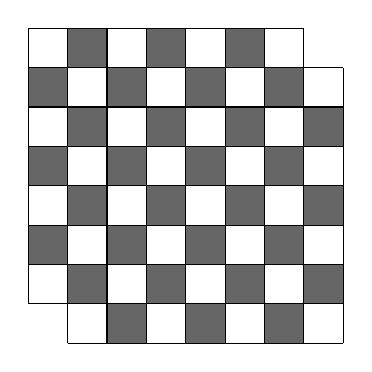
\begin{tikzpicture}[x=0.5cm,y=0.5cm]
  \foreach \i in {0,...,3} 
    \foreach \j in {0,...,3}
    \fill[line width=1pt,color=black,fill=black,fill opacity=0.6] (2*\i,2*\j) -- (2*\i,2*\j+1) -- (2*\i+1,2*\j+1) -- (2*\i+1,2*\j) -- cycle;
  \foreach \i in {0,...,3} 
    \foreach \j in {0,...,3}
        \fill[line width=1pt,color=black,fill=black,fill opacity=0.6] (2*\i+1,2*\j+1) -- (2*\i+1,2*\j+2) -- (2*\i+2,2*\j+2) -- (2*\i+2,2*\j+1) -- cycle;
        \fill[line width=1pt,color=white,fill=white,fill opacity=1] (0,0) -- (0,1) -- (1,1) -- (1,0) -- cycle;
        \fill[line width=1pt,color=white,fill=white,fill opacity=1] (7,7) -- (7,8) -- (8,8) -- (8,7) -- cycle;
    \foreach \i in {1,...,7} \draw[black] (0,\i) -- (8,\i);
    \foreach \i in {1,...,7} \draw[black] (\i,0) -- (\i,8);       
    \draw[black] (1,0) -- (8,0);
    \draw[black] (0,1) -- (0,8);
    \draw[black] (0,8) -- (7,8);
    \draw[black] (8,0) -- (8,7);
  \end{tikzpicture}

Fig. 2

 \end{multicols}
    
 Fig. 3 \hspace{.5cm}
  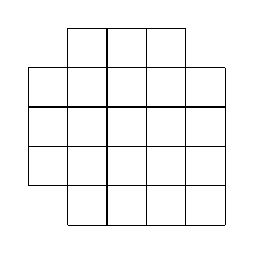
\begin{tikzpicture}[x=0.5cm,y=0.5cm]
     \foreach \i in {1,...,4} \draw[black] (0,\i) -- (5,\i);
    \foreach \i in {1,...,4} \draw[black] (\i,0) -- (\i,5);       
    \draw[black] (1,0) -- (5,0);
    \draw[black] (0,1) -- (0,4);
    \draw[black] (1,5) -- (4,5);
    \draw[black] (5,0) -- (5,4);
  \end{tikzpicture}
  \hspace{3cm} Fig. 4 \hspace{.5cm}  
  
\begin{tikzpicture}[x=0.5cm,y=0.5cm]
     \foreach \i in {0,...,7} \draw[black] (0,\i) -- (7,\i);
    \foreach \i in {0,...,7} \draw[black] (\i,0) -- (\i,7);       
  \end{tikzpicture}
  \\
   
  vi). A un tablero de $(2n)\times (2n)$ se le remueven las cuatro esquinas, como en la Figura 5, donde se ilustra $n=2$, $n=3$ y $n=4$.

¿Para qué valores de $n=2,3,4,5,\dots $ se puede cubrir el resto usando únicamente tetraminos tipo <<$L$>>, sin que se traslapen?

%Sug: i) Algunos se pueden y algunos no se pueden. ii) Para descartar n=2k, colorear con franjas negras y blancas. iii) ¿Es posible cubrir $n=b$ casillas con un número impar de tetraminos <<L>>?
Fig. 5\hspace{.5cm}
  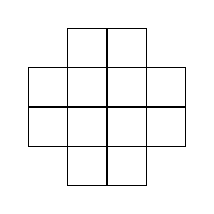
\begin{tikzpicture}[x=0.5cm,y=0.5cm]
     \foreach \i in {1,...,3} \draw[black] (0,\i) -- (4,\i);
    \foreach \i in {1,...,3} \draw[black] (\i,0) -- (\i,4);       
    \draw[black] (1,0) -- (3,0);
    \draw[black] (0,1) -- (0,3);
    \draw[black] (1,4) -- (3,4);
    \draw[black] (4,1) -- (4,3);
  \end{tikzpicture}
  $n=2$
  \hspace{.5cm}  
    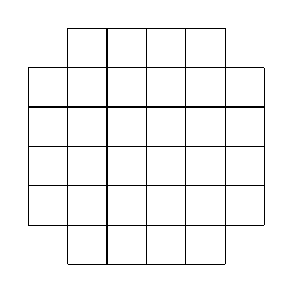
\begin{tikzpicture}[x=0.5cm,y=0.5cm]
     \foreach \i in {1,...,5} \draw[black] (0,\i) -- (6,\i);
    \foreach \i in {1,...,5} \draw[black] (\i,0) -- (\i,6);       
    \draw[black] (1,0) -- (5,0);
    \draw[black] (0,1) -- (0,5);
    \draw[black] (1,6) -- (5,6);
    \draw[black] (6,1) -- (6,5);
  \end{tikzpicture}
  $n=3$
   \hspace{.5cm}
   
\begin{tikzpicture}[x=0.5cm,y=0.5cm]
     \foreach \i in {1,...,7} \draw[black] (0,\i) -- (8,\i);
    \foreach \i in {1,...,7} \draw[black] (\i,0) -- (\i,8);       
    \draw[black] (1,0) -- (7,0);
    \draw[black] (0,1) -- (0,7);
    \draw[black] (1,8) -- (7,8);
    \draw[black] (8,1) -- (8,7);
  \end{tikzpicture}
  $n=4$. 

%Notas al Instructor: i) Ejercicio tipo <<puzzle>>. ii)-iv) Ejemplos de problemas que se justifican con el <<Principio de invarianza>>. En iii) y iv), los más sencillo, siempre hay $n=2+b$ casillas negras y $b$ blancas, pues cada dominó (en cualquier posición) cubre una negra y una blanca. En ii) una cantidad impar de tetraminos <<T>> impiden la construcción (pues no se puede cubrir $n=b$ con un número impar de <<T>>'s). v) Dos posibles coloraciones por diagonales a tres colores. Abreviar casos posibles usando simetrías / modificaciones locales. vi) se requiere un argumento de coloración (por franjas) y un argumento de paridad. 
 
\begin{multicols}{2}
\section*{Áreas}

i). Un triángulo $ABC$ tiene como medidas de sus lados $AB=3$, $AC=4$, y el ángulo $\measuredangle BAC=30^{\circ}$, como en la Figura 1. Calcula el área del triángulo. 

(Pista: $\sen(30^{\circ})=\frac{1}{2}$).\\
%Sug: La altura del triángulo es $h=b\cdot \sen(30^{\circ})$. De hecho, en general, el área de un triángulo es $\frac{1}{2}\cdot b\cdot c \cdot \sen(\apha)$

ii). En un círculo de radio 1 se inscribe un dodecágono regular, como en la Figura 2. Calcula su área.\\
%Sug: ¿Cuál es el área de cada uno de los doce sectores triangulares?.

iii). Calcula ahora el área de un $360$-ágono regular inscrito en un círculo de radio $1$. 

(Pista: $\sen(1^{\circ})=0.0174524$)\\
%Sug: ¿Cuál es el área de cada uno de los $360$ sectores triangulares?.

iv). Calcula el área de caracol de la Figura 3.\\

Los ángulos entre rayos consecutivos desde el centro del caracol son de $30^{\circ}$.\\

Las longitudes de los trece rayos están en progresión aritmética: \\

$l_1=1, l_2=2, l_3=3, \dots, l_{12}=12, l_{13}=13$. 

%Sug: Te puede ayudar la fórmula para el ejercicio x) de aritmética.


\section*{Divisores y residuos}

Un divisor de un número entero $n$ es otro número entero $d$ tal que la fracción $\frac{n}{d}=q$ es igual a otro número entero. En otras palabras $n=d\times q$. 

Por ejemplo, el número $n=6$ tiene cuatro divisores positivos: $d=1,2,3,6$ (pues $\frac{6}{1}=6$, $\frac{6}{2}=3$, $\frac{6}{3}=2$, $\frac{6}{6}=1$, son enteros, pero $\frac{6}{4}=1,5$ y $\frac{6}{5}=1,2$ no lo son).

\columnbreak



Fig.1

\definecolor{uuuuuu}{rgb}{0.26666666666666666,0.26666666666666666,0.26666666666666666}
\definecolor{xdxdff}{rgb}{0.49019607843137253,0.49019607843137253,1}
\definecolor{ududff}{rgb}{0.30196078431372547,0.30196078431372547,1}
\begin{tikzpicture}[line cap=round,line join=round,>=triangle 45,x=2.5cm,y=2.5cm]
\draw [line width=1pt] (0,0)-- (1,0);
\draw[color=black] (0.3,0.1) node {$r=1$};
\draw [line width=1pt] (1,0)-- (0.8660254037844387,0.5);
\draw [line width=1pt] (0.8660254037844387,0.5)-- (0.5,0.8660254037844386);
\draw [line width=1pt] (0.5,0.8660254037844386)-- (0,1);
\draw [line width=1pt] (0,1)-- (-0.5,0.8660254037844386);
\draw [line width=1pt] (-0.5,0.8660254037844386)-- (-0.8660254037844383,0.5);
\draw [line width=1pt] (-0.8660254037844383,0.5)-- (-1,0);
\draw [line width=1pt] (-1,0)-- (-0.8660254037844386,-0.5);
\draw [line width=1pt] (-0.8660254037844386,-0.5)-- (-0.5,-0.8660254037844384);
\draw [line width=1pt] (-0.5,-0.8660254037844384)-- (0,-1);
\draw [line width=1pt] (0,-1)-- (0.5,-0.8660254037844388);
\draw [line width=1pt] (0.5,-0.8660254037844388)-- (0.8660254037844384,-0.5);
\draw [line width=1pt] (0.8660254037844384,-0.5)-- (1,0);
\end{tikzpicture}

Fig. 2

\begin{tikzpicture}[line cap=round,line join=round,>=triangle 45,x=.3cm,y=.3cm]
\draw [line width=1pt] (0,0)-- (1,0);
\draw [line width=1pt] (1,0)-- (1.7320508075688774,1);
\draw [line width=1pt] (1.7320508075688774,1)-- (1.5,2.598076211353316);
\draw [line width=1pt] (1.5,2.598076211353316)-- (0,4);
\draw [line width=1pt] (0,4)-- (-2.5,4.3301270189221945);
\draw [line width=1pt] (-2.5,4.3301270189221945)-- (-5.196152422706631,3);
\draw [line width=1pt] (-5.196152422706631,3)-- (-7,0);
\draw [line width=1pt] (-7,0)-- (-6.928203230275514,-4);
\draw [line width=1pt] (-6.928203230275514,-4)-- (-4.5,-7.794228634059941);
\draw [line width=1pt] (-4.5,-7.794228634059941)-- (0,-10);
\draw [line width=1pt] (0,-10)-- (5.5,-9.526279441628834);
\draw [line width=1pt] (5.5,-9.526279441628834)-- (10.392304845413255,-6);
\draw [line width=1pt] (10.392304845413255,-6)-- (13,0);
\draw [line width=1pt] (0,0)-- (1.7320508075688774,1);
\draw [line width=1pt] (0,0)-- (1.5,2.598076211353316);
\draw [line width=1pt] (0,0)-- (0,4);
\draw [line width=1pt] (0,0)-- (-2.5,4.3301270189221945);
\draw [line width=1pt] (0,0)-- (-5.196152422706631,3);
\draw [line width=1pt] (0,0)-- (-7,0);
\draw [line width=1pt] (0,0)-- (-6.928203230275514,-4);
\draw [line width=1pt] (0,0)-- (-4.5,-7.794228634059941);
\draw [line width=1pt] (0,0)-- (0,-10);
\draw [line width=1pt] (0,0)-- (5.5,-9.526279441628834);
\draw [line width=1pt] (0,0)-- (10.392304845413255,-6);
\draw [line width=1pt] (1,0)-- (13,0);
\draw[color=black] (-4.3475,-4.305) node {$\ddots$};
\draw[color=black] (-1.7575,-6.06) node {$l_{9}=9$};
\draw[color=black] (0.375,-7.635) node {$l_{10}=10$};
\draw[color=black] (5.4875,-5.475) node {$l_{11}=11$};
\draw[color=black] (6.7625,-2.325) node {$l_{12}=12$};
\draw[color=black] (7.3975,0.69) node {$l_{13}=13$};
\end{tikzpicture}

Fig. 3

\end{multicols}

El número $n=18$ tiene seis divisores positivos: $d=1,2,3,6,9,18$. El número $d=7$ no es divisor de $18$, pues $\frac{18}{7}=2+\frac{4}{7}$, no es un entero. El cociente de esa division es $2$ y el residuo es $4$.\\

i). ¿Cuántos divisores positivos tiene $n=360$?\\

ii).  ¿Cuántos divisores positivos tiene $n=10008000$?\\

%Sug: Si n=p_1^{\alpha_1}p_2^{\alpha_2}p_3^{\alpha_3}\cdots p_k^{\alpha_k}. Entonces $n$ tiene exactamente $(\alpha_+1)(\alpha_2+1)(\alpha_3+1)\dots (\alpha_k+1) divisores. ¿Por qué?.

iii). ¿Cuál es el residuo al dividir $100080001$ entre nueve?\\

%Sug: 1+8+1. ¿Por qué? 

iv). ¿Cuál es el residuo al dividir $2021^{2021}+2020^{2020}$ entre nueve?\\

%Sug: Observar cómo se comportan los residuos entre nueve de $2020^1, 2020^2, 2020^3, 2020^4, 2020^5, \dots$. Comparar con $4^1, 4^2, 4^3, 4^4, 4^5, \dots$.

v). Encuentra el menor entero positivo $n$ tal que:
\begin{itemize}
\item al dividir a $n$ entre $7$, sobra $6$,
\item al dividir a $n$ entre $11$, sobra $10$,
\item al dividir a $n$ entre $13$, sobra $12$.
\end{itemize}

%Sug: $7\cdot 11 \cdot 13 =1001$.


\section*{Álgebra}

Te recordamos la expansión y reducción de un binomio, al cuadrado y al cubo ($n=2,3$):
$$(x+y)^2=(x+y)(x+y)=xx+xy+yx+yy= x^2+2xy+y^2,$$
$$(x+y)^3=(x+y)(x+y)(x+y)=\dots = x^3+3x^2y+3xy^2+y^3.$$

i). Considera el binomio a la novena potencia $(x+y)^{9}$. Después de expandir y simplificar términos semejantes.  ¿Cuál es el coeficiente que acompaña a $x^3y^6$?.\\

ii). ¿Cuál es el coeficiente de $x^2y^3z^4$ al simplificar $(x+y+z)^{9}$?.

%Sug: Triángulo de Pascal.

\section*{Probabilidad}

i) Se lanza una moneda siete veces. ¿Cuál es la probabilidad de obtener <<cara>> exactamente cuatro veces?\\

%Sug: El n-ésimo renglón triángulo de Pascal indica las probabilidades de obtener k=0,1,2,\dots n veces <<cara>>. ¿Por qué?. 

ii) ¿Qué evento es más probable: 
Lanzar un dado en doce ocasiones y obtener al menos dos veces <<seis>>, o lanzar un dado seis ocasiones y obtener al menos una vez <<cuatro>>?.\\

iii) Considera el siguiente juego de azar: Lanzas 8 volados...

Si te salen un número par de <<caras>> (es decir, si salen $0,2,4,6$ u $8$), pierdes y pagas $1\$ $. 

Si te salen un número impar de caras ($1,3,5$ o $7$ veces <<cara>>), ganas y te pagan $(1,10)\$ $. 

¿Conviene o no conviene jugar este juego?\\

iv) El juego <<Trez loko>> se juega de la siguiente manera:

Se paga un peso por jugar, y se lanzan diez dados. Te fijas en cuantos <<tres>> obtuviste.

Si lo lograste en tres ocasiones o más, ganas y te pagan $3\$$.

¿Cuál es la probabilidad de ganar?

¿Conviene o no conviene jugar al <<Trez loko>>?

\section*{Trigonometría}

Te recordamos las identidades trigonométricas para sumas de ángulos:
$$\cos(\alpha+\beta)=\cos(\alpha)\cos(\beta)-\sen(\alpha)\sen(\beta), \quad \sen(\alpha+\beta)=\cos(\alpha)\sen(\beta)+\sen(\alpha)\cos(\beta)$$

i) Expresa $\sen(3\alpha)$ y $\cos(3\alpha)$ en términos de $\sen(\alpha)$ y $\cos(\alpha)$.\\

ii). Expresa $\sen(7\alpha)$ y $\cos(6\alpha)$ en términos de $\sen(\alpha)$ y $\cos(\alpha)$.

%Sug: Triángulo de Pascal y números complejos (identidad de Euler).

\section*{Pre-cálculo}

i) ¿Cuánto vale el siguiente límite?:

$$\lim_{n\to\infty}=\frac{n}{2}\sen\left(\frac{2 \pi}{n} \right).$$

%Sug: Problemas ii) y iii) de áreas.

ii) ¿Por qué la derivada de la función $f(x)=x^n$ es $nx^{n-1}$?\\

%Sug: Aplicar el teorema del binomio a $(x+h)^n$

iii) ¿Por qué la derivada de la función $\cos(x)$ es $\sen(x)$ y la derivada de la función $\sen(x)$ es $-\cos(x)$?

